%% LyX 2.2.1 created this file.  For more info, see http://www.lyx.org/.
%% Do not edit unless you really know what you are doing.
\documentclass[12pt]{article}
\usepackage[latin9]{inputenc}
\usepackage[letterpaper]{geometry}
\geometry{verbose}
\usepackage{fancyhdr}
\pagestyle{fancy}
\usepackage{float}
\usepackage{mathtools}
\usepackage{bm}
\usepackage{amsmath}
\usepackage{amssymb}
\usepackage{graphicx}
\usepackage{setspace}
\setstretch{1.5}

\makeatletter
%%%%%%%%%%%%%%%%%%%%%%%%%%%%%% User specified LaTeX commands.


% packages
                   	
\usepackage{bm}
\usepackage[nodisplayskipstretch]{setspace}
\usepackage{enumitem}
\usepackage{fancyheadings}
\usepackage{csquotes}


% Configuration


\input{"../middle_header.txt"}
\chead{Model Building}
\title{\vspace{-1cm}Model  Building Exercises}

% Custom commands
\newif\ifanswers
\answerstrue % comment out to hide answers

\makeatother

\begin{document}
\maketitle

\thispagestyle{fancy}

\section{Motivation}

The ability of Bayesian methods to handle hierarchical models in an
unusually tidy way is why they are becoming the first choice for complex
problems in ecology and conservation biology, problems with multiple
unknowns, sources of data and sources of uncertainty. Recall that
the posterior distribution of all of the unobserved quantities is
proportionate to the joint distributions of the unobserved quantities
and the data:

\[
\big[\bm{\theta}\mid\mathbf{y}\big]\propto\underbrace{\big[\bm{\theta},\mathbf{y}\big]}_{\mathclap{\text{Factor into sensible parts}}}
\]
It follows that the starting point for developing hierarchical models
is to write a properly factored expression for the proportionality
between the posterior and joint distribution of the observed and unobserved
quantities. Properly means that the expression for the factored joint
distribution obeys the chain rule of probability after assumptions
about independence have been made. Bayesian networks, also called
directed acyclic graphs (or, unattractively in my view, DAGs), offer
a way to visually assure that your model does so. This will be true
if there is one unknown and one data set or one hundred unknowns and
ten data sets. This factored expression is all that is required to
specify a \enquote{roll-your-own} MCMC algorithm or to write code
in one of the current software packages that sample from the marginal
posterior distributions, JAGS, STAN, OpenBUGS etc. The expression
for posterior and joint is where you start discussions with statistical
colleagues. It must be included in all papers and proposals using
Bayesian methods because it communicates virtually everything about
where your inferences come from.

Learning to write proper mathematical and statistical expressions
for Bayesian models is 90 percent of the battle of learning how to
do Bayesian analysis. We will return to this battle time and time
again during this course. In this exercise, we begin to learn the
vital skill of model building. The problems increase in difficulty
as we proceed, so it will be important to understand what you did
right and wrong before you proceed to the next problem. In addition
to practice drawing Bayesian networks and writing posterior and joint
distributions, the problems will challenge you to:
\begin{itemize}
\item Choose distributions appropriate for the support of the random variable. 
\item Deftly use moment matching to convert means and standard deviations
to parameters of distributions. 
\item Make inferences on derived quantities.
\end{itemize}

\section{Preliminaries}
\begin{itemize}
\item Review your notes on the Light Limitation of Trees lecture, where
I illustrated several Bayesian models. The problems were chosen to
align with the material covered in lecture.
\item Read Chapters 1.1 (Preview), 6.1-6.21 (What is a Hierarchical model
through Fecundity of spotted owls)\footnote{Note that in box 6.2.3, the $x_{i}$ in panel B should be $x_{ij}$
implying that there are reps of observation of $x_{ij}$ arising from
a distribution with mean $\chi_{i}$.}, 6.2.2 (Controls on nitrous oxide emissions of agricultural soils)
and 10.1 and 10.2 (General approach, and An example of model building)
in Hobbs and Hooten.
\item Do problem 12.1 (Fisher's ticks) and consult the answers after struggling
with each part. No write-up require on this one. It's a warmup.
\end{itemize}

\section{Instructions}
\begin{itemize}
\item For each problem below, draw the Bayesian network, write the posterior
and joint distributions using generic bracket notation with appropriate
products. Next, choose specific distributions following the general
flow that I illustrated in the Light Limitation of Trees lecture.
At this point, don't worry too much about the specific forms for prior
distributions. We will learn more about composing these as the course
proceeds. You may use uniform distributions with bounds that are vague
for non-negative parameters. Use normal distributions centered on
zero with large variances for real-valued parameters. Again, don't
sweat this too much. 
\item Work in groups to allow discussion and to teach each other. Prepare
a write up, one per group. You may use pencil and paper for drawing
DAGs and writing models. I don't want you to struggle with LaTeX at
the same time you are struggling with model building. Scan your drawings
and equations and turn them in as a pdf. The are due Friday, 3/1.
We will go over the problems in class on Tuesday 3/7.
\item I urge you to do a problem as completely as you possibly can, then
consult the answer before going to the next problem. Don't correct
your answer after consulting mine because I need to see how your are
doing. The point is not to get the model right the first time, but
rather to learn by trying to get it right. 
\item If you think you have found a mistake, good for you! There will be
some lurking errors because some of these problems have not been vetted.
There is no better way to show that you are learning than to find
mistakes. 
\item Accumulate questions.
\end{itemize}

\section{Problems}

\subsection{The Kuznets effect}

You are interested in modeling the relationship between per capita
income and an index of air pollution for 80 nations around the world.
You hypothesize that air pollution increases then declines as per
capita income increases (i.e., the Kuznets effect). Choose a deterministic
model to represent this humped relationship. The response, an air
pollution index, and the predictor variable, income, are based on
a sample of observations from each country. You have data on the mean
(and the standard deviation of the mean) for each country's air pollution
index, a continuous, non-negative response variable. You also have
a mean and a standard deviation of the mean for each county's income,
which is also continuous and non-negative. How would you model the
effect of income on air pollution to include uncertainty in the response
and the predictor? \newline Hint \textendash{} Think of the response
and predictor data as arising from distributions of means with known
standard deviations. You want to use the unobserved means of those
distributions in your model of the Kuznets effect.

\ifanswers \newpage{}
\begin{figure}[H]
\center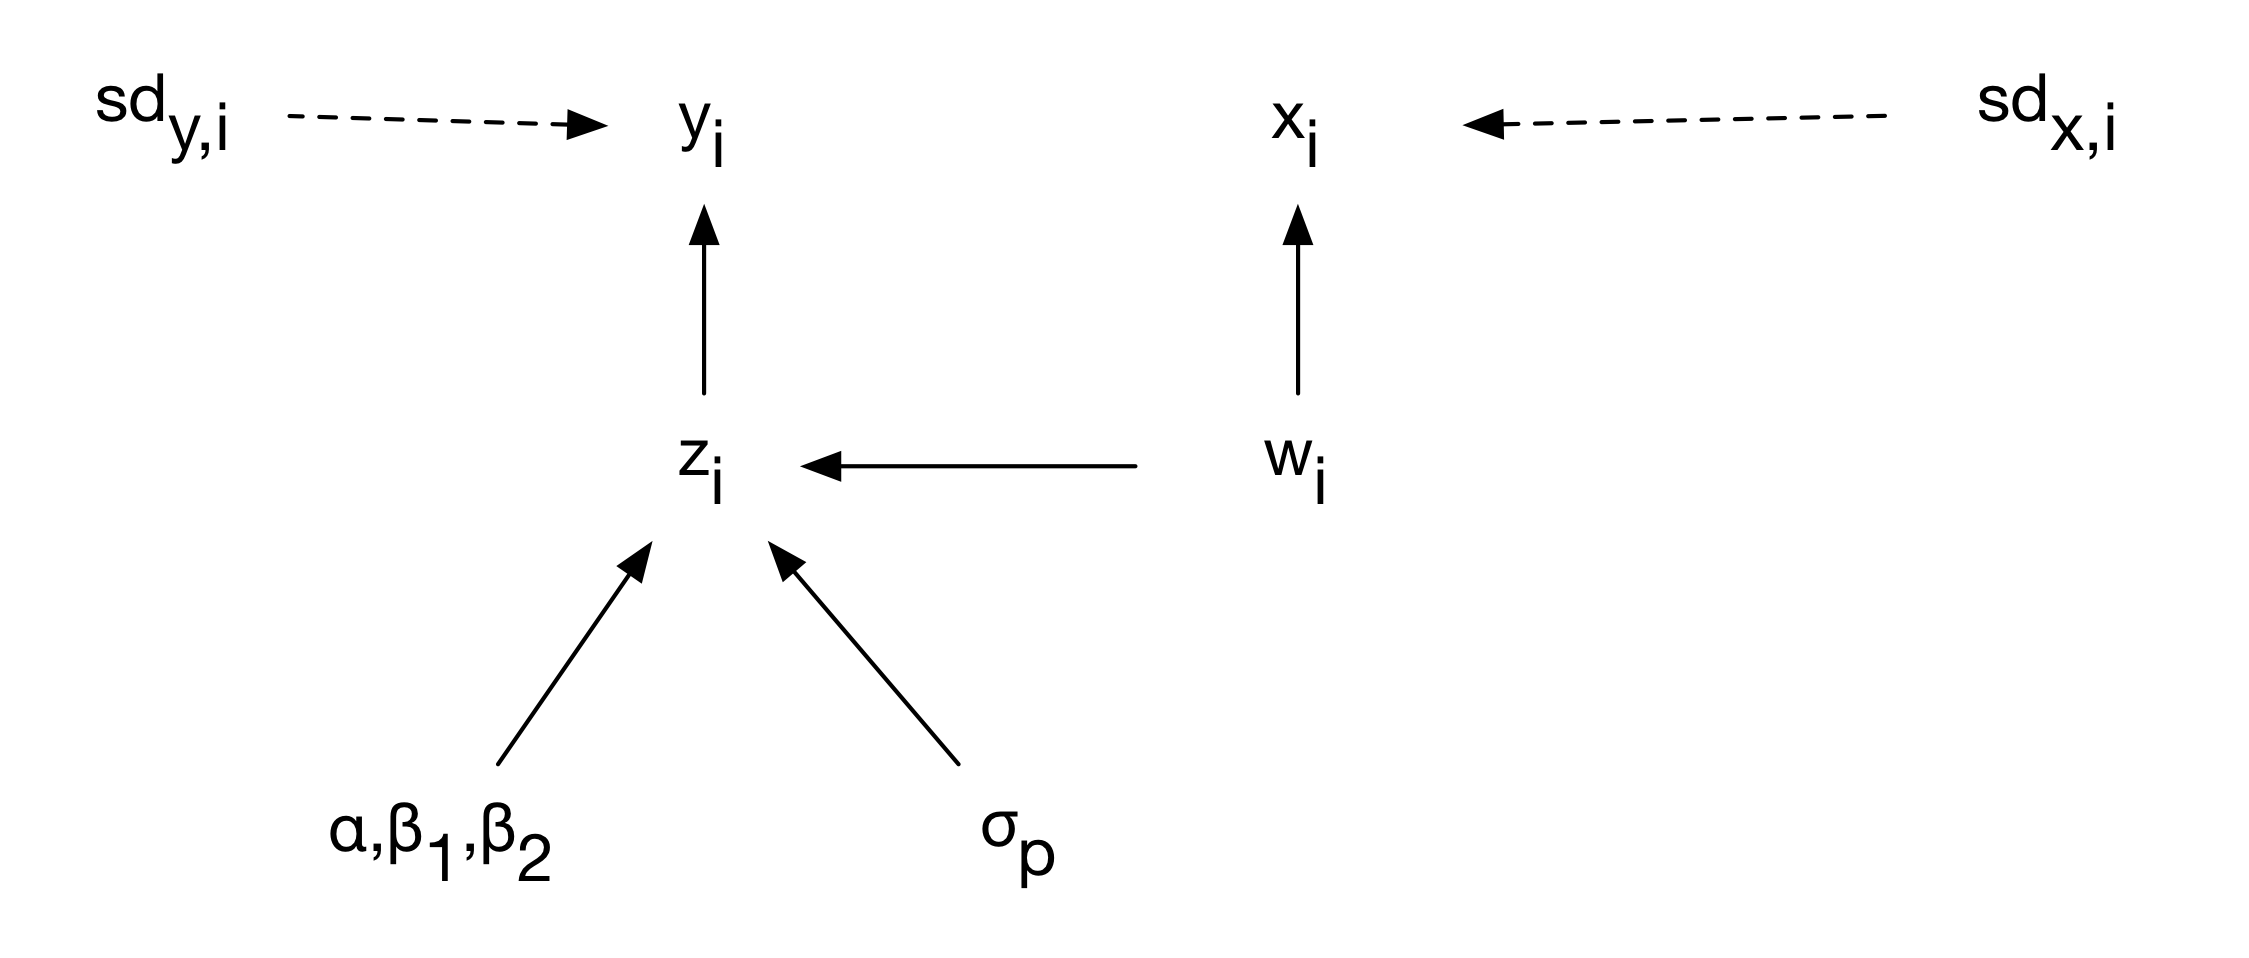
\includegraphics[width=4.75in,bb = 0 0 200 100, draft, type=eps]{../../../../SESYNCBayes/Labs/ModelBuilding/KuznetsDAG.png}
\caption{\foreignlanguage{american}{In this DAG, $y_{i}$ and $sd_{y,i}$ and $x_{i}$ and $sd_{x,i}$
and are the observed means (and standard deviations of the means)
of air quality and per capita income in the $i_{th}$ country. The
observed $y_{i}$ and $x_{i}$ are random variables drawn from distributions
with unobserved mean $z_{i}$ for pollution and unobserved mean $w_{i}$
for income. We assume the standard deviations of those distributions
are known as $sd_{y,i}$ and $sd_{x,i}$.}}
\end{figure}

\begin{align*}
\big[\bm{z},\bm{w},\alpha,\bm{\beta},\sigma_{p}\mid\bm{y},\bm{x}\big]\varpropto & \prod_{i=1}^{n}\big[z_{i}\mid g\big(\alpha,\bm{\beta},w_{i}\big),\sigma_{p}^{2}\big]\big[x_{i}\mid w_{i},sd_{x,i}\big]\big[y_{i}\mid z_{i},sd_{y,i}\big]\\
 & \times\big[w_{i}\big]\big[\alpha\big]\big[\beta_{1}\big]\big[\beta_{2}\big]\big[\sigma_{p}\big]
\end{align*}
\[
\begin{aligned} & g\big(\alpha,\bm{\beta},w_{i}\big)\big)=e^{\alpha+\beta_{1}w_{i}+\beta_{2}w_{i}^{2}}\\
 & z_{i}\sim\textrm{gamma}\left(\frac{g\big(\alpha,\bm{\beta},w_{i}\big)^{2}}{\sigma_{p}^{2}},\frac{g\big(\alpha,\bm{\beta},w_{i}\big)}{\sigma_{p}^{2}}\right)\\
 & y_{i}\sim\textrm{gamma}\left(\frac{z_{i}^{2}}{sd_{y,i}^{2}},\frac{z_{i}}{sd_{y,i}^{2}}\right)\\
 & x_{i}\sim\textrm{gamma}\left(\frac{w_{i}^{2}}{sd_{x,i}^{2}},\frac{w_{i}}{sd_{x,i}^{2}}\right)\\
 & w_{i}\sim\textrm{gamma}\big(.001,.001)
\end{aligned}
\quad\quad\quad\begin{aligned} & \alpha\sim\textrm{normal}\big(0,10000)\\
 & \beta_{1}\sim\textrm{normal}\big(0,10000)\\
 & \beta_{2}\sim\textrm{normal}\big(0,10000)\\
 & \sigma_{p}\sim\textrm{gamma}\big(.001,.001)\\
\\
\end{aligned}
\]

\textbf{Notes:} We use an exponentiated, quadratic model to represent
our hypothesis to assert that the prediction of pollution is a humped
function of income and is strictly non-negative. A linear model (not
exponentiated) would have been a reasonable alternative. We could
have moment matched the lognormal distribution for $z_{i},w_{i}$
and $y_{i}$, but we must be careful to moment match for \emph{both}
parameters in this case. Matching for the mean alone will give the
wrong answer (badly wrong). This is to say that moment matching for
the first parameter using the log of the median would not work. Why?
Because the second parameter is on the log scale and your standard
deviations are on the exponential scale. We also could have used models
like
\begin{eqnarray}
\log(z_{i}) & \sim & \textrm{\text{normal}}\left(\log(g\big(\alpha,\bm{\beta},w_{i}\big)),\sigma_{p}^{2}\right)\\
\log(y_{i}) & \sim & \text{normal}(\log(z_{i}),sd_{y,i}^{2})\\
\log(x_{i}) & \sim & \text{normal}(\log(w_{i}),sd_{x,i}^{2})\\
\end{eqnarray}

You might be tempted to use the data to put informative priors on
$w_{i}$ and $z_{i}$ as in the incorrect Bayesian network below.
This just doesn't work because now the $y_{i}$ are arising from conflicting
distributions, one with parameters $z_{i},sd_{y,i}^{2}$ and the other
with parameters $g(\alpha,\bm{\beta},w_{i}),\sigma^{2}$, leading
to a violation of the chain rule of probability because the $y_{i}$
appear twice on the left hand side of conditioning. You could not
fit this model.

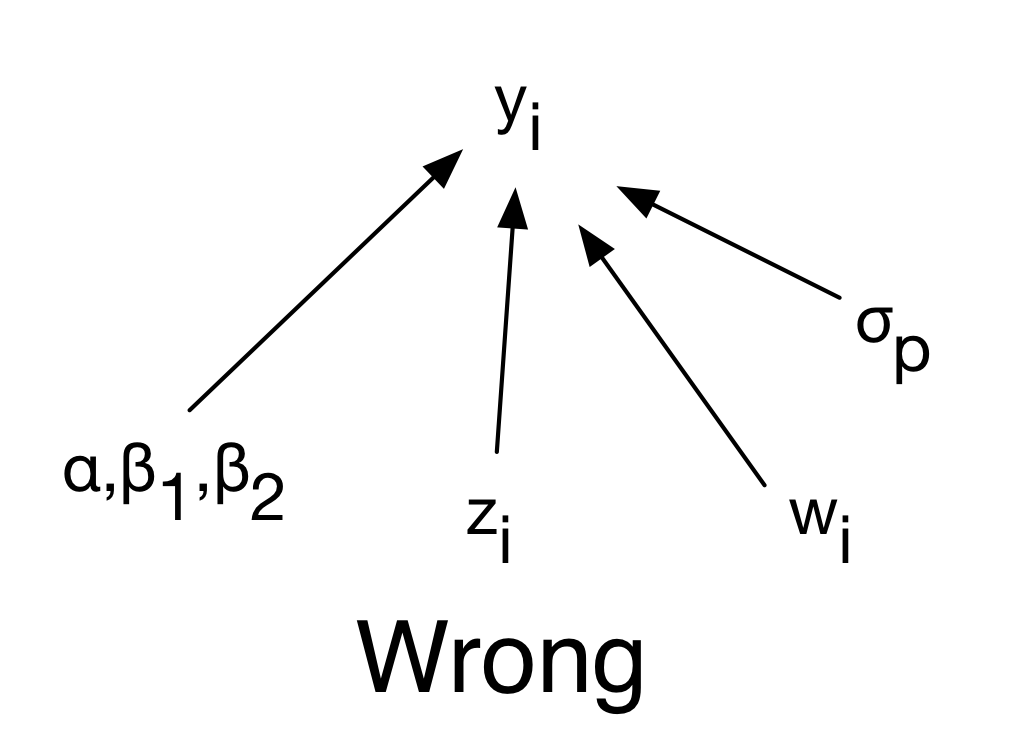
\includegraphics{KuznetsDAGalternative}

\newpage{}\fi

\subsection{Effect of radon on cancer risk}

You seek to understand how radon levels influence risk of cancer.
You have data on the incidence of lung cancer in households (1 if
cancer is present and 0 if no cancer) and radon levels (a continuous,
non-negative number) for 1000 houses in each of 40 counties within
a state. You also have data on the clay soil content at the county
level. You heroically assume both clay content and radon levels are
know without error. How would you model the effect of radon and soil
type on the probability of lung cancer? Some hints\textendash{}
\begin{enumerate}
\item What deterministic model would you use to predict the probability
of cancer in a household as a function of radon level? 
\begin{enumerate}
\item What likelihood would you use for these 0 or 1 data? 
\item Assume that the intercept in your deterministic model of the effect
of radon level on probability of cancer in a household is a linear
function of county level clay soil content.
\end{enumerate}
\ifanswers \newpage{}
\begin{figure}[H]
\center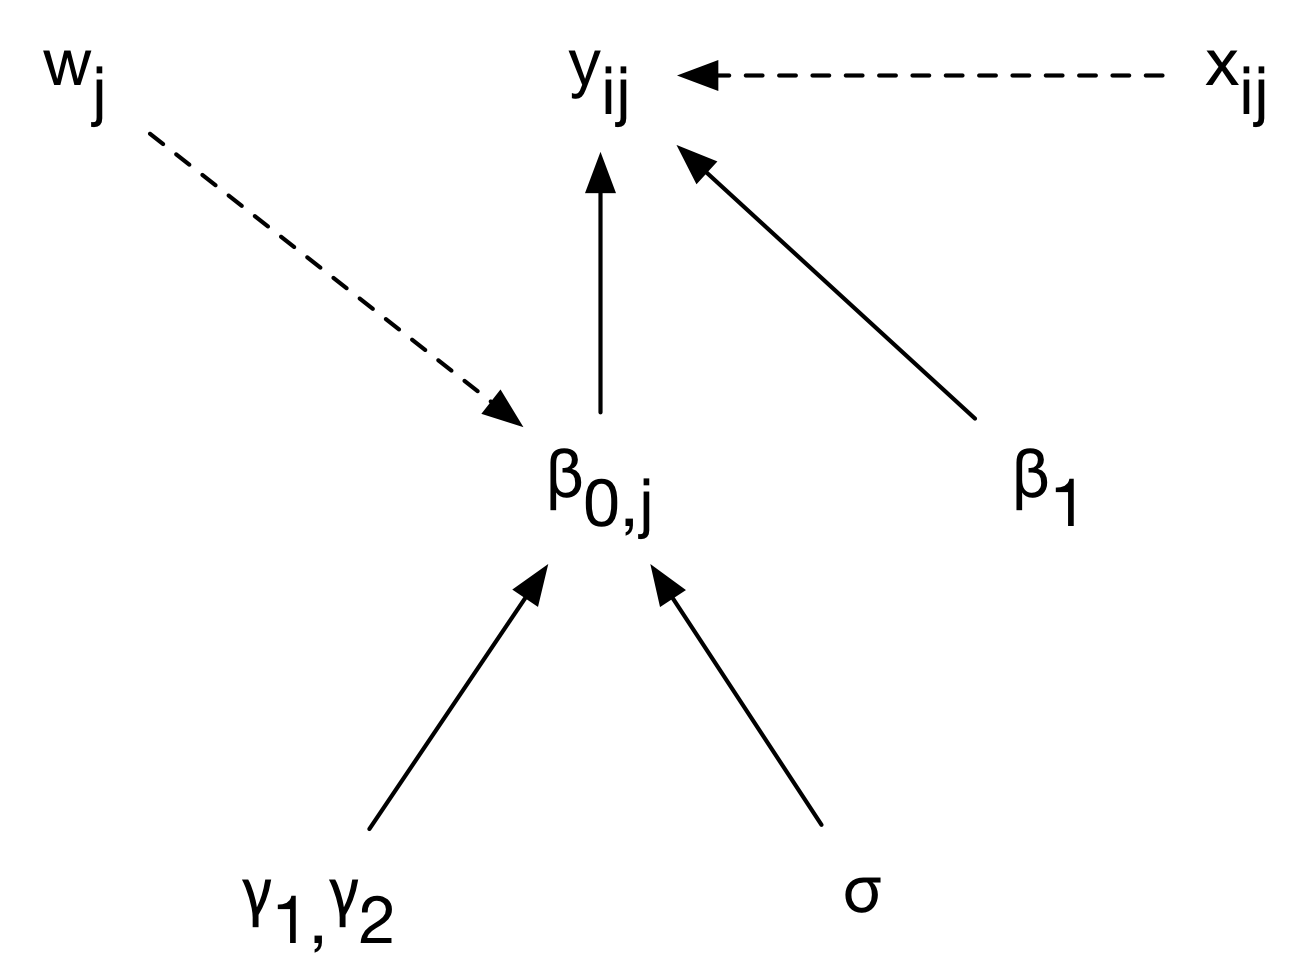
\includegraphics[width=2.75in,bb = 0 0 200 100, draft, type=eps]{../../../../SESYNCBayes/Labs/ModelBuilding/RadonDAG.png}
\caption{In this DAG, $x_{ij}$ is the radon level and $y_{ij}$ is an indicator
that equals 1 if cancer is present and 0 if it is not in the $i_{\textrm{th}}$
house in the $j_{\textrm{th}}$ county, and $w_{\textrm{th}}$ is
the clay soil content in the $j_{\textrm{th}}$ county.}
\end{figure}

\begin{align*}
\big[\bm{\gamma},\bm{\beta},\sigma\mid\bm{y}\big]\varpropto\prod_{i=1}^{1000}\prod_{j=1}^{40}\big[y_{ij}\mid g\big(\bm{\beta},x_{ij}\big)\big]\big[\beta_{0,ij}\mid h\big(\bm{\gamma},w_{j}\big),\sigma^{2}\big]\big[\bm{\gamma}\big]\big[\beta_{1}\big]\big[\sigma\big]
\end{align*}
\[
\begin{aligned} & g\big(\bm{\beta},x_{ij}\big)=\frac{e^{\beta_{0,ij}+\beta_{1}x_{ij}}}{1+e^{\beta_{0,ij}+\beta_{1}x_{ij}}}\\
 & h\big(\bm{\gamma},w_{j}\big)=\gamma_{0}+\gamma_{1}w_{j}\\
 & y_{ij}\sim\textrm{Bernoulli}\big(g\big(\bm{\beta},x_{ij}\big)\big)\\
 & \beta_{0}\sim\textrm{normal}\big(h\big(\bm{\gamma},w_{j}\big),\sigma^{2})\\
 & \beta_{1}\sim\textrm{normal}\big(0,1000)
\end{aligned}
\quad\quad\quad\begin{aligned} & \gamma_{0}\sim\textrm{normal}\big(0,1000)\\
 & \gamma_{1}\sim\textrm{normal}\big(0,1000)\\
 & \sigma\sim\textrm{uniform}\big(0,1000)\\
\\
\\
\end{aligned}
\]
\newpage{}\fi
\end{enumerate}

\subsection{Diversity of a plant community}

You have plot-level data on diversity of plant communities. The data
consist of counts $y_{ij}$ of the number of individuals of species
$i$ on $j=1,\dots,J$ same-sized plots, and the total number of individuals
on plot $j$ is reported as $n_{j}$. How would you model an index
$(H)$ of species diversity across the community, where $H=-\sum_{i=1}^{R}\phi_{i}\textrm{log}\big(\phi_{i}\big)$,
$\phi_{i}$ is the unobserved proportion of the $i_{\textrm{th}}$
species in in the community, and R is the total number of species
present? Hints\textendash{} 
\begin{enumerate}
\item Model the observed count data as a random variable (a vector) arising
from the unobserved vector $\bm{\phi}$ of proportions. 
\item Take a look at the Dirichlet distribution as a way to form an prior
on the vector $\bm{\phi}$. The Dirichlet is to the multinomial likelihood
as the beta distribution is to the binomial likelihood. A vague Dirichlet
has parameters = 1 for all categories. 
\item Calculate $H$ as a derived quantity of the $\phi_{i}$ and $R$,
which will allow us to obtain a posterior distribution for $H$ because
any quantity that is a function of a random variable becomes a random
variable in Bayesian analysis. 

\ifanswers \newpage{}
\begin{figure}[H]
\centering{}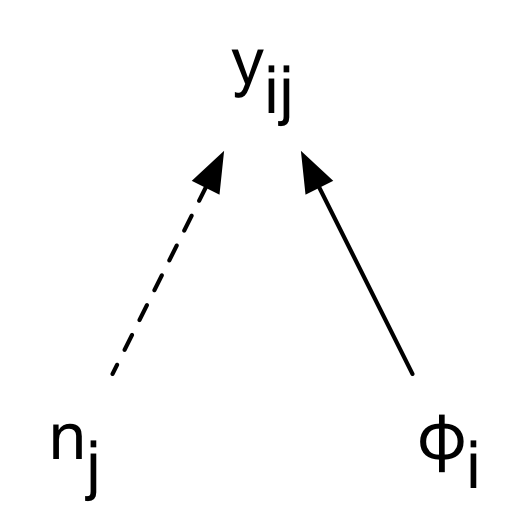
\includegraphics[width=1.5in,bb = 0 0 200 100, draft, type=eps]{../../../../SESYNCBayes/Labs/ModelBuilding/DiversityDAG.png}
\caption{In this DAG, $y_{ij}$ is the number of individuals in the $i_{\textrm{th}}$
species observed in the $j_{\textrm{th}}$ plot while $n_{j}$ is
the total number of individuals across all species observed in the
$j_{\textrm{th}}$ plot. }
\end{figure}

\begin{align*}
\big[\boldsymbol{\phi}\mid\mathbf{Y}\big]\varpropto\prod_{j=1}^{J}\big[\bm{y}_{j}\mid n_{j},\bm{\phi}\big]\big[\bm{\phi}\big]
\end{align*}
\[
\begin{aligned} & H=-\sum_{i=1}^{R}\phi_{i}\textrm{log}\big(\phi_{i}\big)\\
 & \bm{y}_{j}\sim\textrm{multinomial}\big(n_{j},\bm{\phi}\big)\\
 & \bm{\phi}\sim\textrm{Dirichlet}\underbrace{\big(1,1,\cdots,1\big)'}_{\text{a vector of length R}}
\end{aligned}
\]

\vspace{10mm}

where $R$ is the the observed, total number of species across all
plots.\newpage{}\fi
\end{enumerate}

\subsection{Controls on willow seedling establishment}
\begin{enumerate}
\item You are interested in the way that soil water and herbaceous plant
cover influence establishment of willow seedlings in riparian communities.
You have data on the number of willow seedlings that establish on
100 10 $\times$ 10 meter plots. Assume these data are measured perfectly
(i.e., you did not over or under count seedlings). You also have five
measurements of soil water and one measurement of percent herbaceous
cover (estimated visually) on each plot. Assume for now that herbaceous
cover is measured perfectly, but you want to include sampling variation
in soil water for each plot in your model. How would you model the
effect of soil water and herbaceous cover on the number of plants
established?\newpage 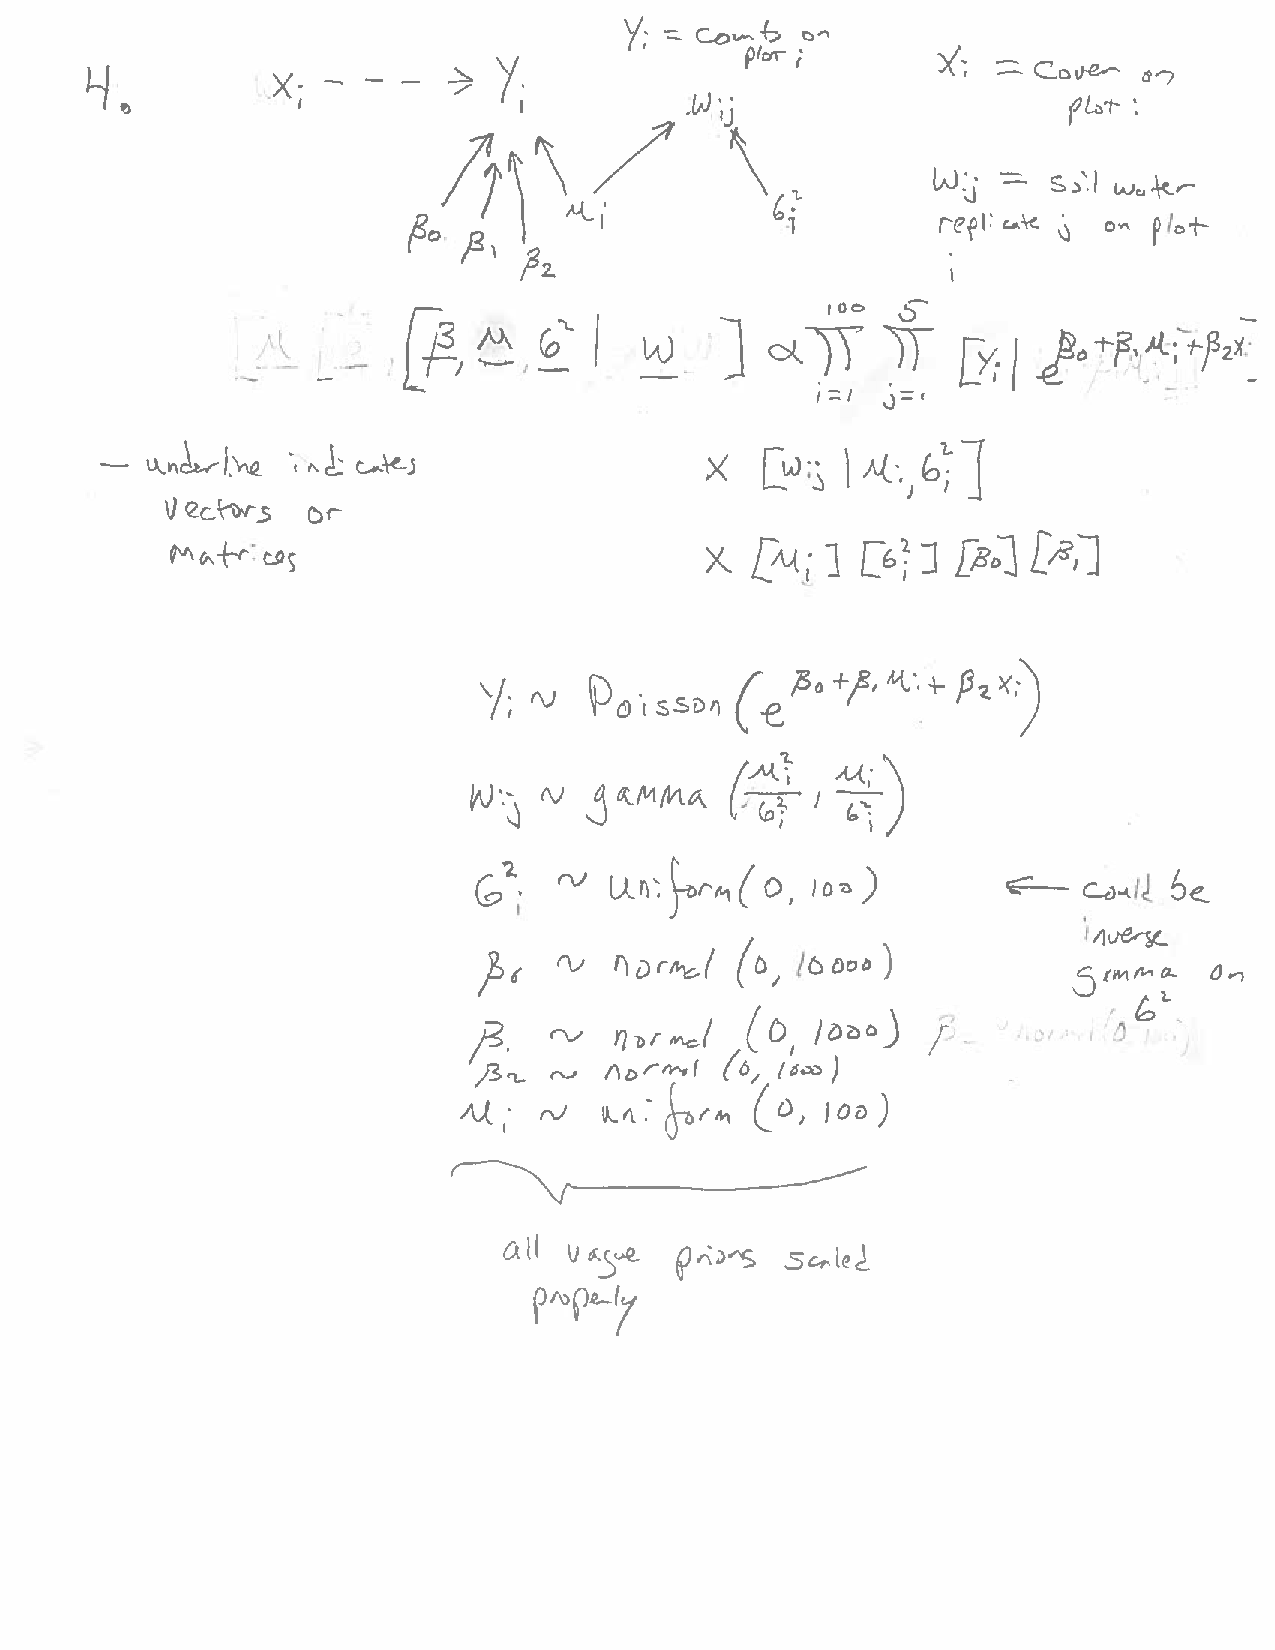
\includegraphics[width=0.9\columnwidth]{AnswerToProb4}
\newpage
\item Your major professor objected to your assumption of cover observed
perfectly by eye, insisting, reasonably I think, that you develop
a data model relating your ocular estimate to the true cover in a
plot. So, you obtained visual estimates of cover paired with the actual
proportion of vegetated area (measured using small sub-plots) on 15
10 x 10 m plots. After days of sweaty labor, you regressed visual
estimates $(x_{i})$ on the true cover $(z_{i})$ and developed a
calibration equation $h(\bm{\alpha},z_{i})$:
\begin{eqnarray}
h(\bm{\alpha},x_{i}) & = & \frac{e^{\alpha_{o}+\alpha_{1}z_{i}}}{1+e^{\alpha_{o}+\alpha_{1}z_{i}}}\\
x_{i} & \sim & \text{beta}\big(m(h(\bm{\alpha},z_{i}),\varsigma^{2})\big)\\
\alpha_{o} & \sim & \text{\text{normal}(.05,.006)}\\
\alpha_{1} & \sim & \text{normal}(1.07,.13)\\
\varsigma^{2} & \sim & \text{inverse gamma}(10.2,630)
\end{eqnarray}
The function $m(\,)$ returns parameters of the beta distribution
given moments as inputs. Include the calibration equation in your
model of effects of soil water and herbaceous cover on seedling establishment
using informed priors on $\alpha_{0},\alpha_{1}$ and $\varsigma^{2}$.
Hint\textendash think about the predictor variable for herbaceous
cover. Do you want to use the observed value of cover $(x_{i})$ or
the true value $(z_{i})$ to model its effect on establishment?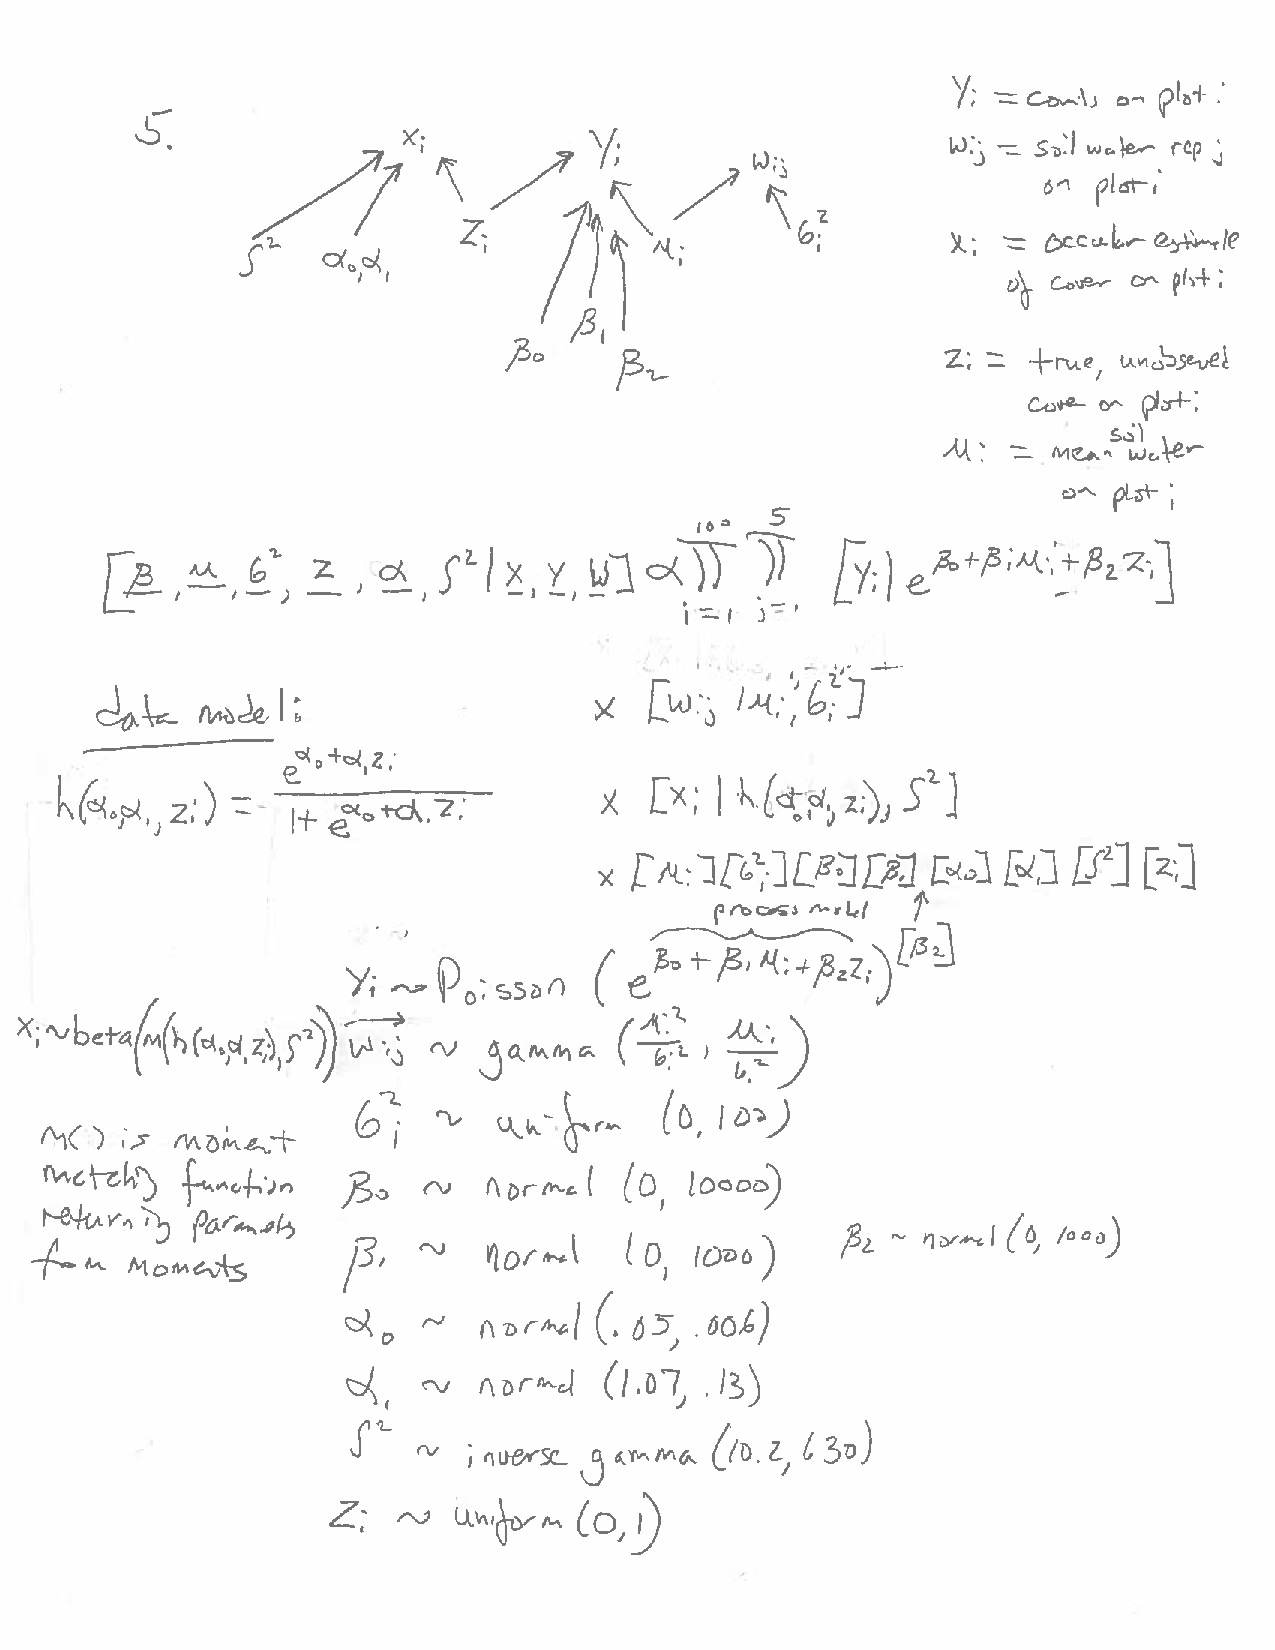
\includegraphics[width=0.9\columnwidth]{AnswerToProb5}
\item Now presume that the 100 plots are arranged in 5 different stream
reaches, 20 plots in each reach. You have data on peak runoff in each
of the reaches, which you may assume is measured perfectly. Describe
verbally how you might model variation at the catchment scale created
by peak runoff. \big skip You could allow each stream reach to have its own intercept
(i.e., $\beta_{0,j}$), which you model as a linear or non-linear
function of data of peak runoff. 
\end{enumerate}

\end{document}
